\documentclass[border=4pt]{standalone}

\usepackage{amsmath}
\usepackage{tikz}
\usepackage{mathdots}
\usepackage{yhmath}
\usepackage{cancel}
\usepackage{color}
\usepackage{siunitx}
\usepackage{array}
\usepackage{multirow}
\usepackage{amssymb}
\usepackage{gensymb}
\usepackage{tabularx}
\usepackage{booktabs}
\usetikzlibrary{fadings}
\usetikzlibrary{patterns}


\begin{document}
 
     

\tikzset{every picture/.style={line width=0.75pt}} %set default line width to 0.75pt        

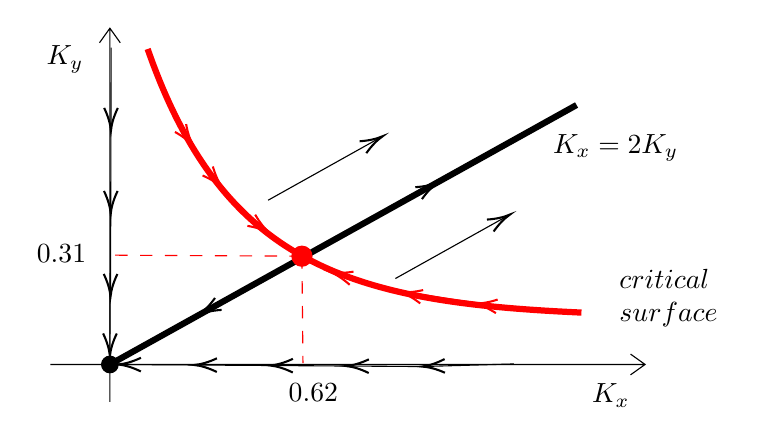
\begin{tikzpicture}[x=0.75pt,y=0.75pt,yscale=-1,xscale=1]
%uncomment if require: \path (0,300); %set diagram left start at 0, and has height of 300

%Shape: Axis 2D [id:dp4854614797684984] 
\draw  (50,229) -- (336.5,229)(78.65,67) -- (78.65,247) (329.5,224) -- (336.5,229) -- (329.5,234) (73.65,74) -- (78.65,67) -- (83.65,74)  ;
%Curve Lines [id:da2066722353902013] 
\draw [color={rgb, 255:red, 255; green, 0; blue, 0 }  ,draw opacity=1 ][line width=2.25]    (96.83,77) .. controls (133.83,183) and (196.83,199) .. (305.83,204) ;


%Straight Lines [id:da10786841723046003] 
\draw [line width=2.25]    (303.5,104) -- (78.65,229) ;


%Shape: Circle [id:dp43413181112860966] 
\draw  [color={rgb, 255:red, 255; green, 0; blue, 0 }  ,draw opacity=1 ][fill={rgb, 255:red, 255; green, 0; blue, 0 }  ,fill opacity=1 ] (166.33,176.83) .. controls (166.33,174.16) and (168.5,172) .. (171.17,172) .. controls (173.84,172) and (176,174.16) .. (176,176.83) .. controls (176,179.5) and (173.84,181.67) .. (171.17,181.67) .. controls (168.5,181.67) and (166.33,179.5) .. (166.33,176.83) -- cycle ;
%Straight Lines [id:da2322381324336189] 
\draw [color={rgb, 255:red, 255; green, 0; blue, 0 }  ,draw opacity=1 ] [dash pattern={on 4.5pt off 4.5pt}]  (171.17,176.83) -- (171.67,228.33) ;


%Straight Lines [id:da40279233182527907] 
\draw [color={rgb, 255:red, 255; green, 0; blue, 0 }  ,draw opacity=1 ] [dash pattern={on 4.5pt off 4.5pt}]  (171.17,176.83) -- (79,176.33) ;


%Shape: Circle [id:dp2774185318711462] 
\draw  [fill={rgb, 255:red, 0; green, 0; blue, 0 }  ,fill opacity=1 ] (74.65,229) .. controls (74.65,226.79) and (76.44,225) .. (78.65,225) .. controls (80.86,225) and (82.65,226.79) .. (82.65,229) .. controls (82.65,231.21) and (80.86,233) .. (78.65,233) .. controls (76.44,233) and (74.65,231.21) .. (74.65,229) -- cycle ;
%Straight Lines [id:da8976102760097826] 
\draw    (78.75,185) -- (78.65,223) ;
\draw [shift={(78.65,225)}, rotate = 270.14] [color={rgb, 255:red, 0; green, 0; blue, 0 }  ][line width=0.75]    (10.93,-3.29) .. controls (6.95,-1.4) and (3.31,-0.3) .. (0,0) .. controls (3.31,0.3) and (6.95,1.4) .. (10.93,3.29)   ;

%Straight Lines [id:da14719191193816084] 
\draw    (79.05,156.33) -- (78.95,194.33) ;
\draw [shift={(78.95,196.33)}, rotate = 270.14] [color={rgb, 255:red, 0; green, 0; blue, 0 }  ][line width=0.75]    (10.93,-3.29) .. controls (6.95,-1.4) and (3.31,-0.3) .. (0,0) .. controls (3.31,0.3) and (6.95,1.4) .. (10.93,3.29)   ;

%Straight Lines [id:da6956681185955156] 
\draw    (79.15,116.33) -- (79.05,154.33) ;
\draw [shift={(79.05,156.33)}, rotate = 270.14] [color={rgb, 255:red, 0; green, 0; blue, 0 }  ][line width=0.75]    (10.93,-3.29) .. controls (6.95,-1.4) and (3.31,-0.3) .. (0,0) .. controls (3.31,0.3) and (6.95,1.4) .. (10.93,3.29)   ;

%Straight Lines [id:da12274081986973018] 
\draw    (79.25,76.33) -- (79.15,114.33) ;
\draw [shift={(79.15,116.33)}, rotate = 270.14] [color={rgb, 255:red, 0; green, 0; blue, 0 }  ][line width=0.75]    (10.93,-3.29) .. controls (6.95,-1.4) and (3.31,-0.3) .. (0,0) .. controls (3.31,0.3) and (6.95,1.4) .. (10.93,3.29)   ;

%Straight Lines [id:da33227445405862843] 
\draw    (119.25,229.25) -- (84.65,229.01) ;
\draw [shift={(82.65,229)}, rotate = 360.39] [color={rgb, 255:red, 0; green, 0; blue, 0 }  ][line width=0.75]    (10.93,-3.29) .. controls (6.95,-1.4) and (3.31,-0.3) .. (0,0) .. controls (3.31,0.3) and (6.95,1.4) .. (10.93,3.29)   ;

%Straight Lines [id:da4725503233600008] 
\draw    (155.85,229.5) -- (121.25,229.26) ;
\draw [shift={(119.25,229.25)}, rotate = 360.39] [color={rgb, 255:red, 0; green, 0; blue, 0 }  ][line width=0.75]    (10.93,-3.29) .. controls (6.95,-1.4) and (3.31,-0.3) .. (0,0) .. controls (3.31,0.3) and (6.95,1.4) .. (10.93,3.29)   ;

%Straight Lines [id:da33418924886080803] 
\draw    (192.45,229.75) -- (157.85,229.51) ;
\draw [shift={(155.85,229.5)}, rotate = 360.39] [color={rgb, 255:red, 0; green, 0; blue, 0 }  ][line width=0.75]    (10.93,-3.29) .. controls (6.95,-1.4) and (3.31,-0.3) .. (0,0) .. controls (3.31,0.3) and (6.95,1.4) .. (10.93,3.29)   ;

%Straight Lines [id:da5445924509307911] 
\draw    (229.05,230) -- (194.45,229.76) ;
\draw [shift={(192.45,229.75)}, rotate = 360.39] [color={rgb, 255:red, 0; green, 0; blue, 0 }  ][line width=0.75]    (10.93,-3.29) .. controls (6.95,-1.4) and (3.31,-0.3) .. (0,0) .. controls (3.31,0.3) and (6.95,1.4) .. (10.93,3.29)   ;

%Straight Lines [id:da9750991555227966] 
\draw    (273.25,228.75) -- (231.05,229.94) ;
\draw [shift={(229.05,230)}, rotate = 358.38] [color={rgb, 255:red, 0; green, 0; blue, 0 }  ][line width=0.75]    (10.93,-3.29) .. controls (6.95,-1.4) and (3.31,-0.3) .. (0,0) .. controls (3.31,0.3) and (6.95,1.4) .. (10.93,3.29)   ;

%Curve Lines [id:da5777786351730516] 
\draw [color={rgb, 255:red, 255; green, 0; blue, 0 }  ,draw opacity=1 ]   (108.75,106.25) .. controls (123.3,136.32) and (136.91,152.28) .. (154.14,164.62) ;
\draw [shift={(155.75,165.75)}, rotate = 214.78] [color={rgb, 255:red, 255; green, 0; blue, 0 }  ,draw opacity=1 ][line width=0.75]    (10.93,-3.29) .. controls (6.95,-1.4) and (3.31,-0.3) .. (0,0) .. controls (3.31,0.3) and (6.95,1.4) .. (10.93,3.29)   ;

%Curve Lines [id:da28440777146226237] 
\draw [color={rgb, 255:red, 255; green, 0; blue, 0 }  ,draw opacity=1 ]   (99.8,85.6) .. controls (114.28,115.52) and (120.93,129.79) .. (131.8,142.61) ;
\draw [shift={(133,144)}, rotate = 228.69] [color={rgb, 255:red, 255; green, 0; blue, 0 }  ,draw opacity=1 ][line width=0.75]    (10.93,-3.29) .. controls (6.95,-1.4) and (3.31,-0.3) .. (0,0) .. controls (3.31,0.3) and (6.95,1.4) .. (10.93,3.29)   ;

%Curve Lines [id:da9344137421474792] 
\draw [color={rgb, 255:red, 255; green, 0; blue, 0 }  ,draw opacity=1 ]   (103.4,93.6) .. controls (114.98,119.08) and (107.94,108.42) .. (117.85,122.38) ;
\draw [shift={(119,124)}, rotate = 234.73] [color={rgb, 255:red, 255; green, 0; blue, 0 }  ,draw opacity=1 ][line width=0.75]    (10.93,-3.29) .. controls (6.95,-1.4) and (3.31,-0.3) .. (0,0) .. controls (3.31,0.3) and (6.95,1.4) .. (10.93,3.29)   ;

%Curve Lines [id:da5010677988145689] 
\draw [color={rgb, 255:red, 255; green, 0; blue, 0 }  ,draw opacity=1 ]   (269,201.2) .. controls (218.04,194.14) and (212.41,192.47) .. (186.23,184.87) ;
\draw [shift={(184.6,184.4)}, rotate = 376.15999999999997] [color={rgb, 255:red, 255; green, 0; blue, 0 }  ,draw opacity=1 ][line width=0.75]    (10.93,-3.29) .. controls (6.95,-1.4) and (3.31,-0.3) .. (0,0) .. controls (3.31,0.3) and (6.95,1.4) .. (10.93,3.29)   ;

%Curve Lines [id:da7563344924271911] 
\draw [color={rgb, 255:red, 255; green, 0; blue, 0 }  ,draw opacity=1 ]   (301,203.6) .. controls (257.1,200.46) and (247.38,200.4) .. (219.9,194.38) ;
\draw [shift={(218.2,194)}, rotate = 372.53] [color={rgb, 255:red, 255; green, 0; blue, 0 }  ,draw opacity=1 ][line width=0.75]    (10.93,-3.29) .. controls (6.95,-1.4) and (3.31,-0.3) .. (0,0) .. controls (3.31,0.3) and (6.95,1.4) .. (10.93,3.29)   ;

%Curve Lines [id:da00014664850010004393] 
\draw [color={rgb, 255:red, 255; green, 0; blue, 0 }  ,draw opacity=1 ]   (301,203.6) .. controls (257.1,200.46) and (284.26,203.47) .. (256,199.83) ;
\draw [shift={(254.2,199.6)}, rotate = 367.31] [color={rgb, 255:red, 255; green, 0; blue, 0 }  ,draw opacity=1 ][line width=0.75]    (10.93,-3.29) .. controls (6.95,-1.4) and (3.31,-0.3) .. (0,0) .. controls (3.31,0.3) and (6.95,1.4) .. (10.93,3.29)   ;

%Straight Lines [id:da9894375621019176] 
\draw    (181.67,172) -- (235.19,142.11) ;
\draw [shift={(236.93,141.13)}, rotate = 510.82] [color={rgb, 255:red, 0; green, 0; blue, 0 }  ][line width=0.75]    (10.93,-3.29) .. controls (6.95,-1.4) and (3.31,-0.3) .. (0,0) .. controls (3.31,0.3) and (6.95,1.4) .. (10.93,3.29)   ;

%Straight Lines [id:da7692542712997135] 
\draw    (216.2,187.6) -- (269.72,157.71) ;
\draw [shift={(271.47,156.73)}, rotate = 510.82] [color={rgb, 255:red, 0; green, 0; blue, 0 }  ][line width=0.75]    (10.93,-3.29) .. controls (6.95,-1.4) and (3.31,-0.3) .. (0,0) .. controls (3.31,0.3) and (6.95,1.4) .. (10.93,3.29)   ;

%Straight Lines [id:da7031274350037] 
\draw    (154.87,149.87) -- (208.39,119.98) ;
\draw [shift={(210.13,119)}, rotate = 510.82] [color={rgb, 255:red, 0; green, 0; blue, 0 }  ][line width=0.75]    (10.93,-3.29) .. controls (6.95,-1.4) and (3.31,-0.3) .. (0,0) .. controls (3.31,0.3) and (6.95,1.4) .. (10.93,3.29)   ;

%Straight Lines [id:da667702452540134] 
\draw    (154.53,186.73) -- (123.08,204.16) ;
\draw [shift={(121.33,205.13)}, rotate = 331] [color={rgb, 255:red, 0; green, 0; blue, 0 }  ][line width=0.75]    (10.93,-3.29) .. controls (6.95,-1.4) and (3.31,-0.3) .. (0,0) .. controls (3.31,0.3) and (6.95,1.4) .. (10.93,3.29)   ;


% Text Node
\draw (320,244) node    {$K_{x}$};
% Text Node
\draw (57,82) node    {$K_{y}$};
% Text Node
\draw (322.33,124.67) node    {$K_{x} =2K_{y}$};
% Text Node
\draw (348,197) node    {$ \begin{array}{l}
critical\ \\
surface
\end{array}$};
% Text Node
\draw (55.33,175.67) node    {$0.31$};
% Text Node
\draw (176.67,242.33) node    {$0.62$};


\end{tikzpicture}
\end{document}
